%! Author = gcpease
%! Date = 4/27/21
\documentclass[border=5mm]{article}
\usepackage{pgfplots}
\usepackage{amsmath}
\usepackage[utf8]{inputenc}
\usepackage[a4paper, total={8in, 10in}]{geometry}
\usepackage{paracol}
\usepackage{titling}
\usetikzlibrary{arrows.meta}
\newcommand{\linespace}{\vspace{1cm}}
\setlength{\columnseprule}{0.2pt}
\usepackage{tikz}

\begin{document}
    \begin{paracol}{2}
        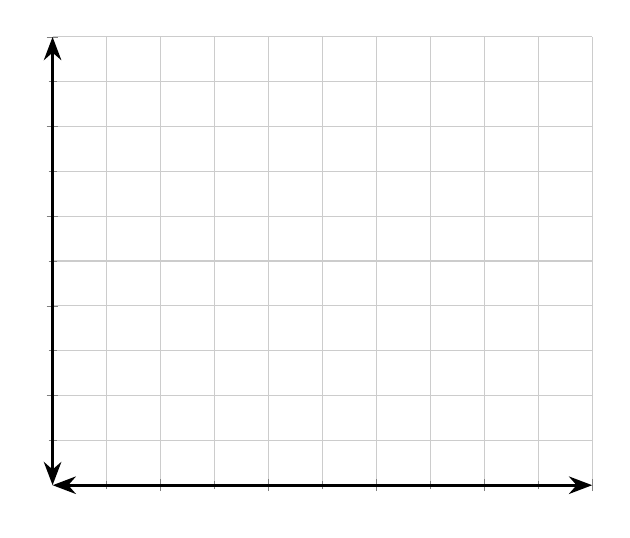
\begin{tikzpicture}[scale=1]
            \begin{axis}[
            axis lines=middle,
            axis line style={Stealth-Stealth,very thick},
            xmin=0,xmax=10,ymin=0,ymax=10,
            minor tick num=1,
            xtick distance=2,
            ytick distance=2,
            xticklabels=,
            yticklabels=,
            grid=both,
            major grid style={thin,black!20},
            minor grid style={thin,black!20}]
            \end{axis}
        \end{tikzpicture}

        \begin{enumerate}
            \item You measured the weight of 10 apples at a store, and found the following weights (in lbs.):

            {
                \centering
                \begin{tabular}{| c | c | c | c | c | c | c | c | c |}
                    \hline
                    1 & $1\frac14$ & 2 & 1 & $1\frac12$ & $1 \frac34$ & 3 & $1\frac14$ & 2 \\[0.5ex]
                    \hline
                \end{tabular}
                
            }

            \begin{enumerate}
                \item Label the X axis.
                \item Label the Y axis.
                \item Plot the data on the graph.
                \item What is the lowest weight? The highest?
                \item What weight is the outlier?
                \item What weight(s) has the most apples?
            \end{enumerate}
        \end{enumerate}
        \linespace
        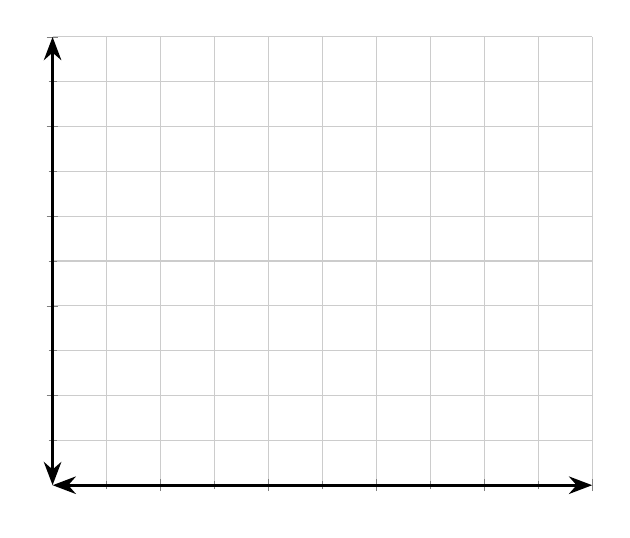
\begin{tikzpicture}[scale=1]
            \begin{axis}[
            axis lines=middle,
            axis line style={Stealth-Stealth,very thick},
            xmin=0,xmax=10,ymin=0,ymax=10,
            minor tick num=1,
            xtick distance=2,
            ytick distance=2,
            xticklabels=,
            yticklabels=,
            grid=both,
            major grid style={thin,black!20},
            minor grid style={thin,black!20}]
            \end{axis}
        \end{tikzpicture}
        \begin{enumerate}
            \setcounter{enumi}{1}
            \item You tracked how much it has rained (in cm) over the past few months. \newline
            {
            \centering
            \begin{tabular}{| c | c | c | c | c | c | c |}
                \hline
                10 & 12 & 10 & 11 & 9 & 8 & 3 \\
                \hline
            \end{tabular}
            }
            \begin{enumerate}
                \item Label the X axis.
                \item Label the Y axis.
                \item Plot the data on the graph.
                \item What is the maximum? The minimum?
                \item What is the difference between the maximum and minimum?
            \end{enumerate}
        \end{enumerate}
        \switchcolumn
        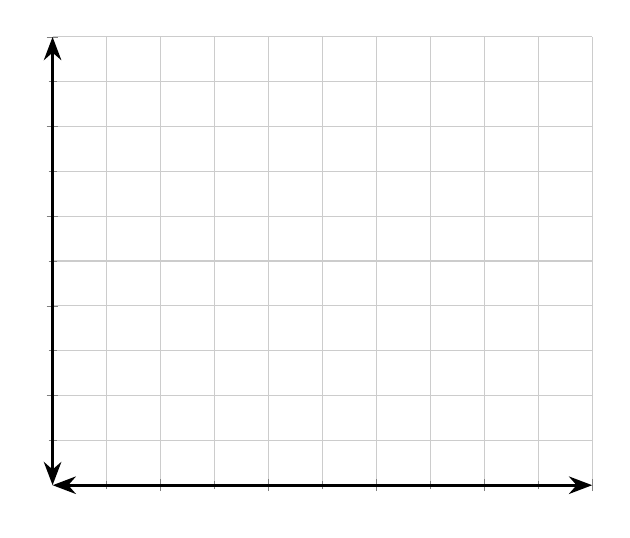
\begin{tikzpicture}[scale=1]
            \begin{axis}[
            axis lines=middle,
            axis line style={Stealth-Stealth,very thick},
            xmin=0,xmax=10,ymin=0,ymax=10,
            minor tick num=1,
            xtick distance=2,
            ytick distance=2,
            xticklabels=Products sold,
            yticklabels=Occurance,
            grid=both,
            major grid style={thin,black!20},
            minor grid style={thin,black!20}]
            \end{axis}
        \end{tikzpicture}
        \begin{enumerate}
            \item Suppose you track how much product a company sells over the course of 8 weeks.\newline\newline
            {\centering
            \begin{tabular}{|c | c | c | c | c | c | c | c|}
                \hline
                Jan & Feb & March & April & May & Jun & Jul & Aug \\
                \hline
                20  & 23  & 15    & 18    & 20  & 20  & 25  & 18  \\
                \hline
            \end{tabular}}
            \newline
            \begin{enumerate}
                \item Plot the data on the graph.
                \item What is the maximum? The minimum?
                \item What is the difference between the maximum and minimum?
                \item What month did the company sell the most products?
            \end{enumerate}
        \end{enumerate}
        \linespace
        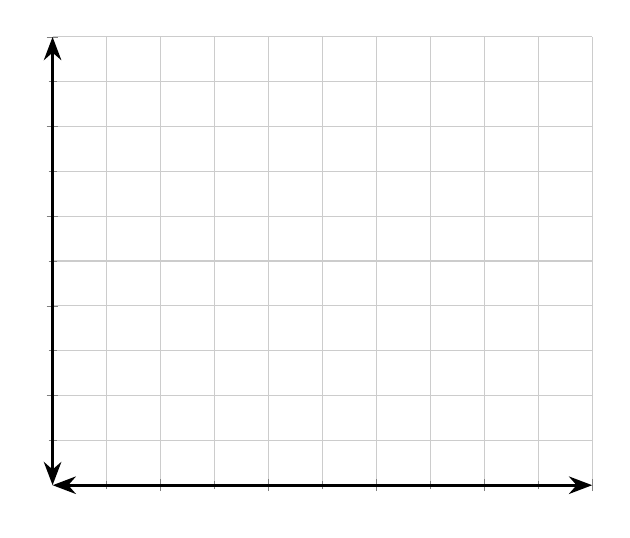
\begin{tikzpicture}[scale=1]
            \begin{axis}[
            axis lines=middle,
            axis line style={Stealth-Stealth,very thick},
            xmin=0,xmax=10,ymin=0,ymax=10,
            minor tick num=1,
            xtick distance=2,
            ytick distance=2,
            xticklabels=Products sold,
            yticklabels=Occurance,
            grid=both,
            major grid style={thin,black!20},
            minor grid style={thin,black!20}]
            \end{axis}
        \end{tikzpicture}
        \begin{enumerate}
            \item You track how much cups of water you drink over a week.\newline
            {
            \centering
            \begin{tabular}{|c | c | c | c | c | c | c |}
                \hline
                1 & 3 & 2 & 9 & 9 & 2 & 4 \\
                \hline
            \end{tabular}
            }
            \newline
            \begin{enumerate}
                \item Plot the data on the graph.
                \item What is the maximum? The minimum?
                \item What is the difference between the maximum and minimum?
                \item How often did you drink 1 cup? 2 cups?
                \item How often did 9 occur out of the set?
            \end{enumerate}
        \end{enumerate}
    \end{paracol}
\end{document}